\documentclass[12 pt]{article}

\usepackage{stoversymb}
\usepackage{fullpage,amsmath,amsfonts,amssymb,url,multicol,graphicx}
%===makes urls render well===
\usepackage{lmodern}
\usepackage[T1]{fontenc}
%============================
\usepackage{wasysym} % smileys
\usepackage[inline]{enumitem}

%,amsthm,amscd,amsbsy,graphpap,makeidx,xfrac,graphicx,floatflt,verbatim,tikz}

%\usetikzlibrary{matrix,arrows}

\everymath{\displaystyle}

\setenumerate{itemsep=0.25in}
\setlist[enumerate,1]{label=\arabic*.}
\setlist[enumerate,2]{label={(\alph*)}}
\setlist[enumerate,3]{label={\roman*.}}

\newcommand{\hint}[1]{\hspace{0.5in}\textbf{Hint}: #1}

\begin{document}
\begin{flushright}Name: \line(1,0){200}\end{flushright}
\begin{center}
\Large{\textbf{MAC 2312 --- Homework 2}}
\end{center}
\textbf{Directions:} Complete the following problems (front and back) for a homework grade. Problems \textit{must} be neatly written up and presented in a professional manner in order to receive credit, and answers given without showing work will not be eligible to receive partial credit. \textbf{Date Due:} October 10, 2016.
\vspace{0.125in}
\begin{enumerate}[leftmargin=0in, rightmargin=-0.25in]
	%========Slack==============
	\item Go to the course's \textsc{Slack} room (see course homepage for the URL) and post something on any one of the channels. You may also create a new channel and comment there.\\[3mm]\hint{One way to grade this question is to assign points based on whether you said something trivial like \textit{Hey!} or \textit{'sup brah} versus something about what you did last weekend, how your classes are going, etc. Participate accordingly.... ;)}
	%========Approx Ints==========
	\item \begin{enumerate}
		\item Given the graph of the function $f(x)=x^2+x+4$ below, sketch the rectangles corresponding to an $M_5$ approximation of $I=\textstyle \int_{-4}^{6}f(x)\,dx$.
		\begin{center}
		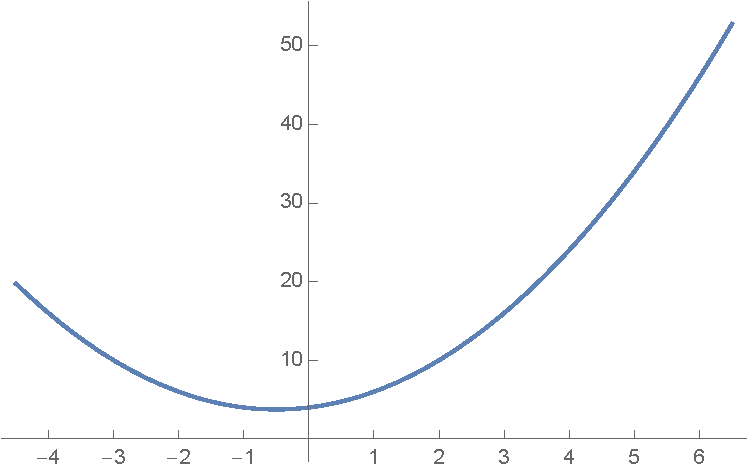
\includegraphics[scale=0.85]{graph}
		\end{center}
		%\newpage
		\item Use $M_5$, $T_5$, and $S_8$ to numerically approximate $I$.
		\item Bound the errors of the three approximations found in part (b).\\[3mm]\hint{You'll need to find $f''$ and $f^{(4)}$ and find the (approximate) maximum of each on the interval $[-4,6]$; these values can be used for $K_1$ and $K_2$, respectively.}
		\item How many trapezoids must be used to ensure that $T_n$ approximates $I$ within an error of $10^{-16}$?
	\end{enumerate}
	%%========Improper Ints=======
	\item \begin{enumerate}
		\item For each of the following integrals, determine whether they're type I improper, type II improper, or not improper at all. Then, determine whether the integral converges or diverges, and if it converges, compute its value.
		\begin{enumerate}[itemsep=0.5in]
			%\item $\int_0^\infty \frac{dx}{x+1}$
			\item $\int_{-\infty}^0 e^x \cos x\,dx$ %\hint{Treat $\lim_{x\to\pm\infty}f(x)$ like a number for $f(x)=\sin(x)\text{ or\,}\cos(x)$.}
			\item $\int_0^1\frac{\ln x}{x^2}\,dx$
			\item $\int_{\pi/2}^{3\pi/2}\frac{2x+4}{(x^2+1)(x^2+4)}\,dx$
			\item $\int_{-\infty}^{\infty}\frac{dx}{x^2+c}$ for $c>0$.
		\end{enumerate}
		\vspace{0.5in}
		\item For each of the following integrals, determine whether they're type I improper, type II improper, or not improper at all, and whether they converge or diverge.
		\begin{enumerate}[itemsep=0.5in]
			\item $\int_0^\pi\sec\theta\,d\theta$
			\item $\int_1^\infty \frac{\ln x}{x^2}\,dx$
			\item $\int_1^2\frac{dx}{x\ln x}$
			\item $\int_{-3}^\infty e^{-x}\arctan^3{x}\,dx$
			%\item $\int_2^5\frac{dx}{(x-3)(x-4)}$
		\end{enumerate}
		\end{enumerate}
\end{enumerate}
\end{document}